\chapter{Sprint 2 : Gestion des utilisateurs }

\section*{Introduction}
Le présent chapitre détaille le deuxième module que nous avons réalisé au cours de notre projet
qui prend le cas d’utilisation "Gestion des utilisateurs". L’étude de ce sprint couvre la l’analyse, lа conception et lа réalisation.

\section{Analyse}
Dans un projet Scrum, pour chaque itération on commence par la phase d’analyse et spécification du sprint. Dans cette phase on représente le diagramme de cas d’utilisation du sprint en cours et le diagramme de séquence système.

\subsection{Diagramme de cas d’utilisation}
Nous présentons ci-dessus le diagramme de cas d’utilisation raffiné qui traite la gestion des utilisateurs des assurances.
Cette gestion consiste à chercher les utilisateurs par leurs:  noms, prénom, email, roles et d'afficher toutes les informations qui sont:\\
-Login\\
-Prénom\\
-Nom\\
-Email\\
-Rôles\\


\begin{figure}[H]
\centering
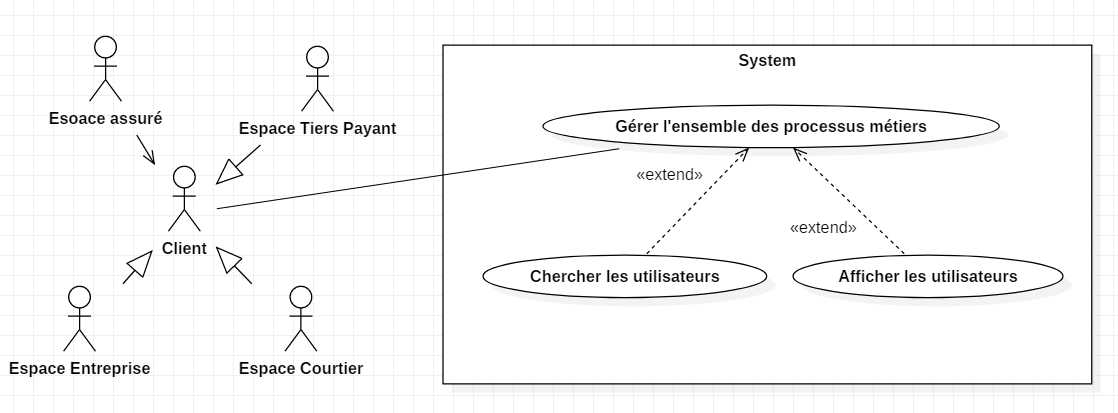
\includegraphics[width=1\columnwidth]{images/useu.PNG}
\caption{Diagramme de cas d'utilisation de gestion des utilisateurs}
\label{fig:Diagramme de cas d'utilisation sprint 1}
\end{figure}

\subsection{Diagramme de séquence système}
Les diagrammes séquence système représentent l’enchaînement dynamique d’un cas d’utilisation: Gestion des utilisateurs
\begin{figure}[H]
\centering
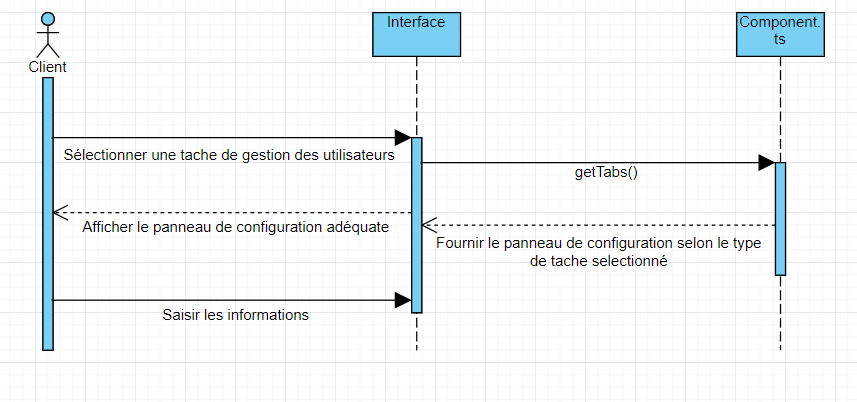
\includegraphics[width=1\columnwidth]{images/seq2.PNG}
\caption{Diagramme de séquences de gestion des utilisateurs des assurances}
\label{fig:Diagramme de cas d'utilisation sprint 1}
\end{figure}






\section{IHM}
\begin{figure}[H]
\centering
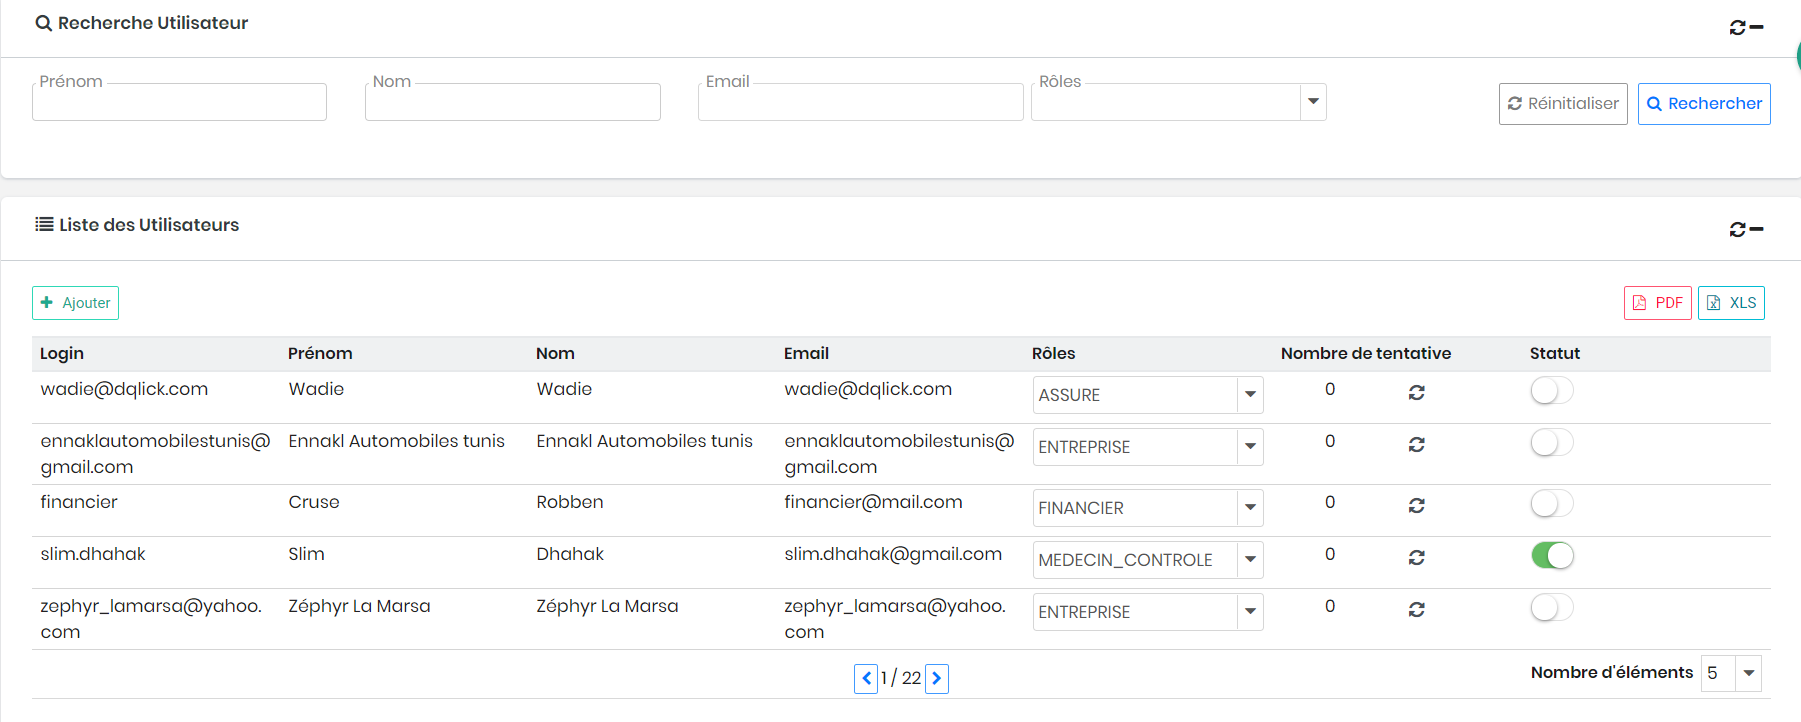
\includegraphics[width=1\columnwidth]{images/interface3.PNG}
\caption{Interface des recherches des utilisateurs}
\label{fig:Diagramme de cas d'utilisation sprint 1}
\end{figure}





\section*{Conclusion}
Dans ce chapitre nous avons réussi à mettre en place une interface de gestions des utilisateus. En effet, le client peut effectuer la recherches des utilisateurs en introduisant leurs informations personnelles et leurs roles.